\documentclass[1p]{elsarticle_modified}
%\bibliographystyle{elsarticle-num}

%\usepackage[colorlinks]{hyperref}
%\usepackage{abbrmath_seonhwa} %\Abb, \Ascr, \Acal ,\Abf, \Afrak
\usepackage{amsfonts}
\usepackage{amssymb}
\usepackage{amsmath}
\usepackage{amsthm}
\usepackage{scalefnt}
\usepackage{amsbsy}
\usepackage{kotex}
\usepackage{caption}
\usepackage{subfig}
\usepackage{color}
\usepackage{graphicx}
\usepackage{xcolor} %% white, black, red, green, blue, cyan, magenta, yellow
\usepackage{float}
\usepackage{setspace}
\usepackage{hyperref}

\usepackage{tikz}
\usetikzlibrary{arrows}

\usepackage{multirow}
\usepackage{array} % fixed length table
\usepackage{hhline}

%%%%%%%%%%%%%%%%%%%%%
\makeatletter
\renewcommand*\env@matrix[1][\arraystretch]{%
	\edef\arraystretch{#1}%
	\hskip -\arraycolsep
	\let\@ifnextchar\new@ifnextchar
	\array{*\c@MaxMatrixCols c}}
\makeatother %https://tex.stackexchange.com/questions/14071/how-can-i-increase-the-line-spacing-in-a-matrix
%%%%%%%%%%%%%%%

\usepackage[normalem]{ulem}

\newcommand{\msout}[1]{\ifmmode\text{\sout{\ensuremath{#1}}}\else\sout{#1}\fi}
%SOURCE: \msout is \stkout macro in https://tex.stackexchange.com/questions/20609/strikeout-in-math-mode

\newcommand{\cancel}[1]{
	\ifmmode
	{\color{red}\msout{#1}}
	\else
	{\color{red}\sout{#1}}
	\fi
}

\newcommand{\add}[1]{
	{\color{blue}\uwave{#1}}
}

\newcommand{\replace}[2]{
	\ifmmode
	{\color{red}\msout{#1}}{\color{blue}\uwave{#2}}
	\else
	{\color{red}\sout{#1}}{\color{blue}\uwave{#2}}
	\fi
}

\newcommand{\Sol}{\mathcal{S}} %segment
\newcommand{\D}{D} %diagram
\newcommand{\A}{\mathcal{A}} %arc


%%%%%%%%%%%%%%%%%%%%%%%%%%%%%5 test

\def\sl{\operatorname{\textup{SL}}(2,\Cbb)}
\def\psl{\operatorname{\textup{PSL}}(2,\Cbb)}
\def\quan{\mkern 1mu \triangleright \mkern 1mu}

\theoremstyle{definition}
\newtheorem{thm}{Theorem}[section]
\newtheorem{prop}[thm]{Proposition}
\newtheorem{lem}[thm]{Lemma}
\newtheorem{ques}[thm]{Question}
\newtheorem{cor}[thm]{Corollary}
\newtheorem{defn}[thm]{Definition}
\newtheorem{exam}[thm]{Example}
\newtheorem{rmk}[thm]{Remark}
\newtheorem{alg}[thm]{Algorithm}

\newcommand{\I}{\sqrt{-1}}
\begin{document}

%\begin{frontmatter}
%
%\title{Boundary parabolic representations of knots up to 8 crossings}
%
%%% Group authors per affiliation:
%\author{Yunhi Cho} 
%\address{Department of Mathematics, University of Seoul, Seoul, Korea}
%\ead{yhcho@uos.ac.kr}
%
%
%\author{Seonhwa Kim} %\fnref{s_kim}}
%\address{Center for Geometry and Physics, Institute for Basic Science, Pohang, 37673, Korea}
%\ead{ryeona17@ibs.re.kr}
%
%\author{Hyuk Kim}
%\address{Department of Mathematical Sciences, Seoul National University, Seoul 08826, Korea}
%\ead{hyukkim@snu.ac.kr}
%
%\author{Seokbeom Yoon}
%\address{Department of Mathematical Sciences, Seoul National University, Seoul, 08826,  Korea}
%\ead{sbyoon15@snu.ac.kr}
%
%\begin{abstract}
%We find all boundary parabolic representation of knots up to 8 crossings.
%
%\end{abstract}
%\begin{keyword}
%    \MSC[2010] 57M25 
%\end{keyword}
%
%\end{frontmatter}

%\linenumbers
%\tableofcontents
%
\newcommand\colored[1]{\textcolor{white}{\rule[-0.35ex]{0.8em}{1.4ex}}\kern-0.8em\color{red} #1}%
%\newcommand\colored[1]{\textcolor{white}{ #1}\kern-2.17ex	\textcolor{white}{ #1}\kern-1.81ex	\textcolor{white}{ #1}\kern-2.15ex\color{red}#1	}

{\Large $\underline{12a_{0035}~(K12a_{0035})}$}

\setlength{\tabcolsep}{10pt}
\renewcommand{\arraystretch}{1.6}
\vspace{1cm}\begin{tabular}{m{100pt}>{\centering\arraybackslash}m{274pt}}
\multirow{5}{120pt}{
	\centering
	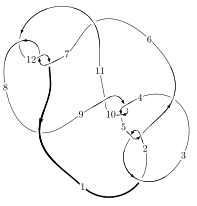
\includegraphics[width=112pt]{../../../GIT/diagram.site/Diagrams/png/836_12a_0035.png}\\
\ \ \ A knot diagram\footnotemark}&
\allowdisplaybreaks
\textbf{Linearized knot diagam} \\
\cline{2-2}
 &
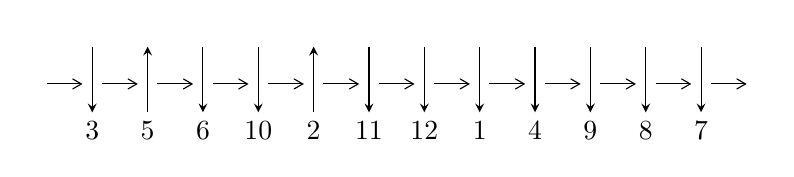
\begin{tikzpicture}[x=20pt, y=17pt]
	% nodes
	\node (C0) at (0, 0) {};
	\node (C1) at (1, 0) {};
	\node (C1U) at (1, +1) {};
	\node (C1D) at (1, -1) {3};

	\node (C2) at (2, 0) {};
	\node (C2U) at (2, +1) {};
	\node (C2D) at (2, -1) {5};

	\node (C3) at (3, 0) {};
	\node (C3U) at (3, +1) {};
	\node (C3D) at (3, -1) {6};

	\node (C4) at (4, 0) {};
	\node (C4U) at (4, +1) {};
	\node (C4D) at (4, -1) {10};

	\node (C5) at (5, 0) {};
	\node (C5U) at (5, +1) {};
	\node (C5D) at (5, -1) {2};

	\node (C6) at (6, 0) {};
	\node (C6U) at (6, +1) {};
	\node (C6D) at (6, -1) {11};

	\node (C7) at (7, 0) {};
	\node (C7U) at (7, +1) {};
	\node (C7D) at (7, -1) {12};

	\node (C8) at (8, 0) {};
	\node (C8U) at (8, +1) {};
	\node (C8D) at (8, -1) {1};

	\node (C9) at (9, 0) {};
	\node (C9U) at (9, +1) {};
	\node (C9D) at (9, -1) {4};

	\node (C10) at (10, 0) {};
	\node (C10U) at (10, +1) {};
	\node (C10D) at (10, -1) {9};

	\node (C11) at (11, 0) {};
	\node (C11U) at (11, +1) {};
	\node (C11D) at (11, -1) {8};

	\node (C12) at (12, 0) {};
	\node (C12U) at (12, +1) {};
	\node (C12D) at (12, -1) {7};
	\node (C13) at (13, 0) {};

	% arrows
	\draw[->,>={angle 60}]
	(C0) edge (C1) (C1) edge (C2) (C2) edge (C3) (C3) edge (C4) (C4) edge (C5) (C5) edge (C6) (C6) edge (C7) (C7) edge (C8) (C8) edge (C9) (C9) edge (C10) (C10) edge (C11) (C11) edge (C12) (C12) edge (C13) ;	\draw[->,>=stealth]
	(C1U) edge (C1D) (C2D) edge (C2U) (C3U) edge (C3D) (C4U) edge (C4D) (C5D) edge (C5U) (C6U) edge (C6D) (C7U) edge (C7D) (C8U) edge (C8D) (C9U) edge (C9D) (C10U) edge (C10D) (C11U) edge (C11D) (C12U) edge (C12D) ;
	\end{tikzpicture} \\
\hhline{~~} \\& 
\textbf{Solving Sequence} \\ \cline{2-2} 
 &
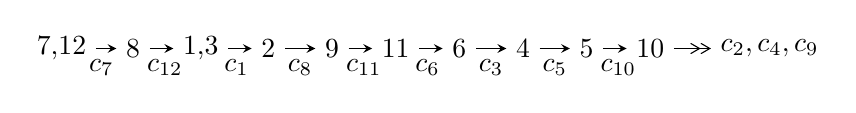
\begin{tikzpicture}[x=23pt, y=7pt]
	% node
	\node (A0) at (-1/8, 0) {7,12};
	\node (A1) at (1, 0) {8};
	\node (A2) at (33/16, 0) {1,3};
	\node (A3) at (25/8, 0) {2};
	\node (A4) at (33/8, 0) {9};
	\node (A5) at (41/8, 0) {11};
	\node (A6) at (49/8, 0) {6};
	\node (A7) at (57/8, 0) {4};
	\node (A8) at (65/8, 0) {5};
	\node (A9) at (73/8, 0) {10};
	\node (C1) at (1/2, -1) {$c_{7}$};
	\node (C2) at (3/2, -1) {$c_{12}$};
	\node (C3) at (21/8, -1) {$c_{1}$};
	\node (C4) at (29/8, -1) {$c_{8}$};
	\node (C5) at (37/8, -1) {$c_{11}$};
	\node (C6) at (45/8, -1) {$c_{6}$};
	\node (C7) at (53/8, -1) {$c_{3}$};
	\node (C8) at (61/8, -1) {$c_{5}$};
	\node (C9) at (69/8, -1) {$c_{10}$};
	\node (A10) at (11, 0) {$c_{2},c_{4},c_{9}$};

	% edge
	\draw[->,>=stealth]	
	(A0) edge (A1) (A1) edge (A2) (A2) edge (A3) (A3) edge (A4) (A4) edge (A5) (A5) edge (A6) (A6) edge (A7) (A7) edge (A8) (A8) edge (A9) ;
	\draw[->>,>={angle 60}]	
	(A9) edge (A10);
\end{tikzpicture} \\ 

\end{tabular} \\

\footnotetext{
The image of knot diagram is generated by the software ``\textbf{Draw programme}" developed by Andrew Bartholomew(\url{http://www.layer8.co.uk/maths/draw/index.htm\#Running-draw}), where we modified some parts for our purpose(\url{https://github.com/CATsTAILs/LinksPainter}).
}\phantom \\ \newline 
\centering \textbf{Ideals for irreducible components\footnotemark of $X_{\text{par}}$} 
 
\begin{align*}
I^u_{1}&=\langle 
-6 u^{93}-19 u^{92}+\cdots+2 b+4,\;3 u^{93}+15 u^{92}+\cdots+2 a-8,\;u^{94}+3 u^{93}+\cdots-4 u-1\rangle \\
I^u_{2}&=\langle 
- u^2 a+b,\;u^2 a+a^2+u^2+a- u+2,\;u^3- u^2+2 u-1\rangle \\
\\
\end{align*}
\raggedright * 2 irreducible components of $\dim_{\mathbb{C}}=0$, with total 100 representations.\\
\footnotetext{All coefficients of polynomials are rational numbers. But the coefficients are sometimes approximated in decimal forms when there is not enough margin.}
\newpage
\renewcommand{\arraystretch}{1}
\centering \section*{I. $I^u_{1}= \langle -6 u^{93}-19 u^{92}+\cdots+2 b+4,\;3 u^{93}+15 u^{92}+\cdots+2 a-8,\;u^{94}+3 u^{93}+\cdots-4 u-1 \rangle$}
\flushleft \textbf{(i) Arc colorings}\\
\begin{tabular}{m{7pt} m{180pt} m{7pt} m{180pt} }
\flushright $a_{7}=$&$\begin{pmatrix}1\\0\end{pmatrix}$ \\
\flushright $a_{12}=$&$\begin{pmatrix}0\\u\end{pmatrix}$ \\
\flushright $a_{8}=$&$\begin{pmatrix}1\\u^2\end{pmatrix}$ \\
\flushright $a_{1}=$&$\begin{pmatrix}- u\\u\end{pmatrix}$ \\
\flushright $a_{3}=$&$\begin{pmatrix}-\frac{3}{2} u^{93}-\frac{15}{2} u^{92}+\cdots+\frac{29}{2} u+4\\3 u^{93}+\frac{19}{2} u^{92}+\cdots-\frac{17}{2} u-2\end{pmatrix}$ \\
\flushright $a_{2}=$&$\begin{pmatrix}-\frac{1}{2} u^{93}-\frac{3}{2} u^{92}+\cdots-\frac{47}{2} u^2+\frac{17}{2} u\\\frac{1}{2} u^{92}+u^{91}+\cdots-7 u^2+\frac{3}{2} u\end{pmatrix}$ \\
\flushright $a_{9}=$&$\begin{pmatrix}- u^4- u^2+1\\u^4+2 u^2\end{pmatrix}$ \\
\flushright $a_{11}=$&$\begin{pmatrix}u\\u^3+u\end{pmatrix}$ \\
\flushright $a_{6}=$&$\begin{pmatrix}- u^4- u^2+1\\- u^6-2 u^4- u^2\end{pmatrix}$ \\
\flushright $a_{4}=$&$\begin{pmatrix}- u^{93}-9 u^{92}+\cdots+18 u+\frac{9}{2}\\\frac{9}{2} u^{93}+15 u^{92}+\cdots-17 u-\frac{9}{2}\end{pmatrix}$ \\
\flushright $a_{5}=$&$\begin{pmatrix}u^{93}+3 u^{92}+\cdots-4 u-\frac{1}{2}\\-\frac{3}{2} u^{93}-3 u^{92}+\cdots-2 u-\frac{3}{2}\end{pmatrix}$ \\
\flushright $a_{10}=$&$\begin{pmatrix}u^{11}+4 u^9+4 u^7-2 u^5-3 u^3+2 u\\- u^{11}-5 u^9-8 u^7-3 u^5+3 u^3+u\end{pmatrix}$\\&\end{tabular}
\flushleft \textbf{(ii) Obstruction class $= -1$}\\~\\
\flushleft \textbf{(iii) Cusp Shapes $= 2 u^{93}+\frac{15}{2} u^{92}+\cdots-\frac{33}{2} u-\frac{11}{2}$}\\~\\
\newpage\renewcommand{\arraystretch}{1}
\flushleft \textbf{(iv) u-Polynomials at the component}\newline \\
\begin{tabular}{m{50pt}|m{274pt}}
Crossings & \hspace{64pt}u-Polynomials at each crossing \\
\hline $$\begin{aligned}c_{1}\end{aligned}$$&$\begin{aligned}
&u^{94}+44 u^{93}+\cdots-9 u+1
\end{aligned}$\\
\hline $$\begin{aligned}c_{2},c_{5}\end{aligned}$$&$\begin{aligned}
&u^{94}+4 u^{93}+\cdots+9 u+1
\end{aligned}$\\
\hline $$\begin{aligned}c_{3}\end{aligned}$$&$\begin{aligned}
&u^{94}-4 u^{93}+\cdots-3441 u+306
\end{aligned}$\\
\hline $$\begin{aligned}c_{4},c_{9}\end{aligned}$$&$\begin{aligned}
&u^{94}+u^{93}+\cdots-160 u-64
\end{aligned}$\\
\hline $$\begin{aligned}c_{6},c_{8}\end{aligned}$$&$\begin{aligned}
&u^{94}+3 u^{93}+\cdots-33 u-34
\end{aligned}$\\
\hline $$\begin{aligned}c_{7},c_{11},c_{12}\end{aligned}$$&$\begin{aligned}
&u^{94}-3 u^{93}+\cdots+4 u-1
\end{aligned}$\\
\hline $$\begin{aligned}c_{10}\end{aligned}$$&$\begin{aligned}
&u^{94}+35 u^{93}+\cdots+66560 u+4096
\end{aligned}$\\
\hline
\end{tabular}\\~\\
\newpage\renewcommand{\arraystretch}{1}
\flushleft \textbf{(v) Riley Polynomials at the component}\newline \\
\begin{tabular}{m{50pt}|m{274pt}}
Crossings & \hspace{64pt}Riley Polynomials at each crossing \\
\hline $$\begin{aligned}c_{1}\end{aligned}$$&$\begin{aligned}
&y^{94}+16 y^{93}+\cdots-369 y+1
\end{aligned}$\\
\hline $$\begin{aligned}c_{2},c_{5}\end{aligned}$$&$\begin{aligned}
&y^{94}+44 y^{93}+\cdots-9 y+1
\end{aligned}$\\
\hline $$\begin{aligned}c_{3}\end{aligned}$$&$\begin{aligned}
&y^{94}-12 y^{93}+\cdots-6463449 y+93636
\end{aligned}$\\
\hline $$\begin{aligned}c_{4},c_{9}\end{aligned}$$&$\begin{aligned}
&y^{94}-35 y^{93}+\cdots-66560 y+4096
\end{aligned}$\\
\hline $$\begin{aligned}c_{6},c_{8}\end{aligned}$$&$\begin{aligned}
&y^{94}-53 y^{93}+\cdots-12309 y+1156
\end{aligned}$\\
\hline $$\begin{aligned}c_{7},c_{11},c_{12}\end{aligned}$$&$\begin{aligned}
&y^{94}+79 y^{93}+\cdots-16 y+1
\end{aligned}$\\
\hline $$\begin{aligned}c_{10}\end{aligned}$$&$\begin{aligned}
&y^{94}+37 y^{93}+\cdots-336592896 y+16777216
\end{aligned}$\\
\hline
\end{tabular}\\~\\
\newpage\flushleft \textbf{(vi) Complex Volumes and Cusp Shapes}
$$\begin{array}{c|c|c}  
\text{Solutions to }I^u_{1}& \I (\text{vol} + \sqrt{-1}CS) & \text{Cusp shape}\\
 \hline 
\begin{aligned}
u &= -0.351586 + 1.054580 I \\
a &= -1.15398 + 1.86992 I \\
b &= \phantom{-}0.313058 - 0.701062 I\end{aligned}
 & -1.40013 - 8.27926 I & \phantom{-0.000000 } 0 \\ \hline\begin{aligned}
u &= -0.351586 - 1.054580 I \\
a &= -1.15398 - 1.86992 I \\
b &= \phantom{-}0.313058 + 0.701062 I\end{aligned}
 & -1.40013 + 8.27926 I & \phantom{-0.000000 } 0 \\ \hline\begin{aligned}
u &= -0.319387 + 1.064870 I \\
a &= \phantom{-}0.60014 - 1.46592 I \\
b &= -0.269640 + 0.910868 I\end{aligned}
 & \phantom{-}0.91044 - 3.19835 I & \phantom{-0.000000 } 0 \\ \hline\begin{aligned}
u &= -0.319387 - 1.064870 I \\
a &= \phantom{-}0.60014 + 1.46592 I \\
b &= -0.269640 - 0.910868 I\end{aligned}
 & \phantom{-}0.91044 + 3.19835 I & \phantom{-0.000000 } 0 \\ \hline\begin{aligned}
u &= \phantom{-}0.272022 + 1.136290 I \\
a &= \phantom{-}1.42508 + 2.49568 I \\
b &= -0.66890 - 1.54095 I\end{aligned}
 & \phantom{-}0.75736 + 2.48496 I & \phantom{-0.000000 } 0 \\ \hline\begin{aligned}
u &= \phantom{-}0.272022 - 1.136290 I \\
a &= \phantom{-}1.42508 - 2.49568 I \\
b &= -0.66890 + 1.54095 I\end{aligned}
 & \phantom{-}0.75736 - 2.48496 I & \phantom{-0.000000 } 0 \\ \hline\begin{aligned}
u &= -0.341633 + 1.119760 I \\
a &= \phantom{-}0.36104 + 1.97232 I \\
b &= \phantom{-}0.355067 - 1.058820 I\end{aligned}
 & -3.79950 - 0.44484 I & \phantom{-0.000000 } 0 \\ \hline\begin{aligned}
u &= -0.341633 - 1.119760 I \\
a &= \phantom{-}0.36104 - 1.97232 I \\
b &= \phantom{-}0.355067 + 1.058820 I\end{aligned}
 & -3.79950 + 0.44484 I & \phantom{-0.000000 } 0 \\ \hline\begin{aligned}
u &= -0.805155 + 0.159834 I \\
a &= -0.683311 - 0.812685 I \\
b &= \phantom{-}2.10771 - 0.56090 I\end{aligned}
 & -4.13551 + 12.51930 I & -12.4410 - 9.1338 I \\ \hline\begin{aligned}
u &= -0.805155 - 0.159834 I \\
a &= -0.683311 + 0.812685 I \\
b &= \phantom{-}2.10771 + 0.56090 I\end{aligned}
 & -4.13551 - 12.51930 I & -12.4410 + 9.1338 I\\
 \hline 
 \end{array}$$\newpage$$\begin{array}{c|c|c}  
\text{Solutions to }I^u_{1}& \I (\text{vol} + \sqrt{-1}CS) & \text{Cusp shape}\\
 \hline 
\begin{aligned}
u &= -0.819292 + 0.023297 I \\
a &= -0.557966 - 0.104325 I \\
b &= \phantom{-}2.01706 - 1.04963 I\end{aligned}
 & -9.72584 + 4.11008 I & -17.4683 - 3.8689 I \\ \hline\begin{aligned}
u &= -0.819292 - 0.023297 I \\
a &= -0.557966 + 0.104325 I \\
b &= \phantom{-}2.01706 + 1.04963 I\end{aligned}
 & -9.72584 - 4.11008 I & -17.4683 + 3.8689 I \\ \hline\begin{aligned}
u &= -0.223727 + 1.159260 I \\
a &= \phantom{-}0.038821 - 0.996676 I \\
b &= -0.793555 + 1.158040 I\end{aligned}
 & \phantom{-}2.56110 - 0.96081 I & \phantom{-0.000000 } 0 \\ \hline\begin{aligned}
u &= -0.223727 - 1.159260 I \\
a &= \phantom{-}0.038821 + 0.996676 I \\
b &= -0.793555 - 1.158040 I\end{aligned}
 & \phantom{-}2.56110 + 0.96081 I & \phantom{-0.000000 } 0 \\ \hline\begin{aligned}
u &= -0.800713 + 0.124544 I \\
a &= \phantom{-}0.056147 - 0.232819 I \\
b &= \phantom{-}1.45417 + 0.99662 I\end{aligned}
 & -6.82446 + 4.61345 I & -16.0257 - 3.7320 I \\ \hline\begin{aligned}
u &= -0.800713 - 0.124544 I \\
a &= \phantom{-}0.056147 + 0.232819 I \\
b &= \phantom{-}1.45417 - 0.99662 I\end{aligned}
 & -6.82446 - 4.61345 I & -16.0257 + 3.7320 I \\ \hline\begin{aligned}
u &= -0.791562 + 0.153666 I \\
a &= \phantom{-}0.673326 + 0.346910 I \\
b &= -1.43596 + 0.24106 I\end{aligned}
 & -1.85813 + 7.30815 I & -9.64546 - 5.45633 I \\ \hline\begin{aligned}
u &= -0.791562 - 0.153666 I \\
a &= \phantom{-}0.673326 - 0.346910 I \\
b &= -1.43596 - 0.24106 I\end{aligned}
 & -1.85813 - 7.30815 I & -9.64546 + 5.45633 I \\ \hline\begin{aligned}
u &= -0.795310\phantom{ +0.000000I} \\
a &= \phantom{-}0.653225\phantom{ +0.000000I} \\
b &= -1.34153\phantom{ +0.000000I}\end{aligned}
 & -6.33214\phantom{ +0.000000I} & -13.9450\phantom{ +0.000000I} \\ \hline\begin{aligned}
u &= \phantom{-}0.207009 + 1.187620 I \\
a &= -0.54176 - 1.63085 I \\
b &= \phantom{-}0.28783 + 1.45505 I\end{aligned}
 & \phantom{-}2.77826 - 1.83941 I & \phantom{-0.000000 } 0\\
 \hline 
 \end{array}$$\newpage$$\begin{array}{c|c|c}  
\text{Solutions to }I^u_{1}& \I (\text{vol} + \sqrt{-1}CS) & \text{Cusp shape}\\
 \hline 
\begin{aligned}
u &= \phantom{-}0.207009 - 1.187620 I \\
a &= -0.54176 + 1.63085 I \\
b &= \phantom{-}0.28783 - 1.45505 I\end{aligned}
 & \phantom{-}2.77826 + 1.83941 I & \phantom{-0.000000 } 0 \\ \hline\begin{aligned}
u &= \phantom{-}0.763490 + 0.126859 I \\
a &= \phantom{-}0.996501 - 0.724536 I \\
b &= -2.36823 - 0.61181 I\end{aligned}
 & -2.24813 - 6.31785 I & -11.54818 + 5.93405 I \\ \hline\begin{aligned}
u &= \phantom{-}0.763490 - 0.126859 I \\
a &= \phantom{-}0.996501 + 0.724536 I \\
b &= -2.36823 + 0.61181 I\end{aligned}
 & -2.24813 + 6.31785 I & -11.54818 - 5.93405 I \\ \hline\begin{aligned}
u &= \phantom{-}0.361057 + 0.671513 I \\
a &= -0.862756 + 0.799832 I \\
b &= -1.113130 - 0.534733 I\end{aligned}
 & -0.51313 - 8.14873 I & -8.97384 + 8.84166 I \\ \hline\begin{aligned}
u &= \phantom{-}0.361057 - 0.671513 I \\
a &= -0.862756 - 0.799832 I \\
b &= -1.113130 + 0.534733 I\end{aligned}
 & -0.51313 + 8.14873 I & -8.97384 - 8.84166 I \\ \hline\begin{aligned}
u &= -0.246747 + 1.213070 I \\
a &= -0.344077 + 0.628748 I \\
b &= \phantom{-}1.32614 - 0.49237 I\end{aligned}
 & \phantom{-}1.93636 + 4.08463 I & \phantom{-0.000000 } 0 \\ \hline\begin{aligned}
u &= -0.246747 - 1.213070 I \\
a &= -0.344077 - 0.628748 I \\
b &= \phantom{-}1.32614 + 0.49237 I\end{aligned}
 & \phantom{-}1.93636 - 4.08463 I & \phantom{-0.000000 } 0 \\ \hline\begin{aligned}
u &= -0.742646 + 0.133805 I \\
a &= \phantom{-}0.305512 - 0.849898 I \\
b &= -0.247171 - 0.370551 I\end{aligned}
 & -0.40083 + 4.55861 I & -9.48261 - 6.77535 I \\ \hline\begin{aligned}
u &= -0.742646 - 0.133805 I \\
a &= \phantom{-}0.305512 + 0.849898 I \\
b &= -0.247171 + 0.370551 I\end{aligned}
 & -0.40083 - 4.55861 I & -9.48261 + 6.77535 I \\ \hline\begin{aligned}
u &= \phantom{-}0.745684 + 0.058825 I \\
a &= \phantom{-}0.284002 - 0.610144 I \\
b &= -1.55723 + 1.53202 I\end{aligned}
 & -4.01862 + 0.63484 I & -14.7380 - 0.8437 I\\
 \hline 
 \end{array}$$\newpage$$\begin{array}{c|c|c}  
\text{Solutions to }I^u_{1}& \I (\text{vol} + \sqrt{-1}CS) & \text{Cusp shape}\\
 \hline 
\begin{aligned}
u &= \phantom{-}0.745684 - 0.058825 I \\
a &= \phantom{-}0.284002 + 0.610144 I \\
b &= -1.55723 - 1.53202 I\end{aligned}
 & -4.01862 - 0.63484 I & -14.7380 + 0.8437 I \\ \hline\begin{aligned}
u &= \phantom{-}0.297640 + 1.220630 I \\
a &= -0.91602 + 3.00986 I \\
b &= \phantom{-}0.17095 - 2.37493 I\end{aligned}
 & -0.46784 - 4.41267 I & \phantom{-0.000000 } 0 \\ \hline\begin{aligned}
u &= \phantom{-}0.297640 - 1.220630 I \\
a &= -0.91602 - 3.00986 I \\
b &= \phantom{-}0.17095 + 2.37493 I\end{aligned}
 & -0.46784 + 4.41267 I & \phantom{-0.000000 } 0 \\ \hline\begin{aligned}
u &= \phantom{-}0.730077 + 0.133883 I \\
a &= -0.875274 + 0.280144 I \\
b &= \phantom{-}1.370320 + 0.318322 I\end{aligned}
 & -0.21470 - 1.60724 I & -7.97056 + 1.57129 I \\ \hline\begin{aligned}
u &= \phantom{-}0.730077 - 0.133883 I \\
a &= -0.875274 - 0.280144 I \\
b &= \phantom{-}1.370320 - 0.318322 I\end{aligned}
 & -0.21470 + 1.60724 I & -7.97056 - 1.57129 I \\ \hline\begin{aligned}
u &= -0.717097 + 0.108393 I \\
a &= \phantom{-}0.308251 + 1.174220 I \\
b &= \phantom{-}0.130133 + 0.598547 I\end{aligned}
 & -1.35579 - 0.62536 I & -12.06986 - 1.95150 I \\ \hline\begin{aligned}
u &= -0.717097 - 0.108393 I \\
a &= \phantom{-}0.308251 - 1.174220 I \\
b &= \phantom{-}0.130133 - 0.598547 I\end{aligned}
 & -1.35579 + 0.62536 I & -12.06986 + 1.95150 I \\ \hline\begin{aligned}
u &= \phantom{-}0.293385 + 0.658021 I \\
a &= \phantom{-}0.266291 - 0.707620 I \\
b &= \phantom{-}0.598578 + 0.548638 I\end{aligned}
 & \phantom{-}1.60349 - 3.29234 I & -5.23174 + 4.77747 I \\ \hline\begin{aligned}
u &= \phantom{-}0.293385 - 0.658021 I \\
a &= \phantom{-}0.266291 + 0.707620 I \\
b &= \phantom{-}0.598578 - 0.548638 I\end{aligned}
 & \phantom{-}1.60349 + 3.29234 I & -5.23174 - 4.77747 I \\ \hline\begin{aligned}
u &= -0.365972 + 1.235490 I \\
a &= -2.15333 + 1.40823 I \\
b &= \phantom{-}1.72605 - 0.32067 I\end{aligned}
 & -5.98368 + 0.15479 I & \phantom{-0.000000 } 0\\
 \hline 
 \end{array}$$\newpage$$\begin{array}{c|c|c}  
\text{Solutions to }I^u_{1}& \I (\text{vol} + \sqrt{-1}CS) & \text{Cusp shape}\\
 \hline 
\begin{aligned}
u &= -0.365972 - 1.235490 I \\
a &= -2.15333 - 1.40823 I \\
b &= \phantom{-}1.72605 + 0.32067 I\end{aligned}
 & -5.98368 - 0.15479 I & \phantom{-0.000000 } 0 \\ \hline\begin{aligned}
u &= \phantom{-}0.658370 + 0.267531 I \\
a &= -0.199386 + 1.344550 I \\
b &= -0.308441 + 0.617622 I\end{aligned}
 & -1.88023 + 4.47482 I & -11.92967 - 3.68864 I \\ \hline\begin{aligned}
u &= \phantom{-}0.658370 - 0.267531 I \\
a &= -0.199386 - 1.344550 I \\
b &= -0.308441 - 0.617622 I\end{aligned}
 & -1.88023 - 4.47482 I & -11.92967 + 3.68864 I \\ \hline\begin{aligned}
u &= \phantom{-}0.146043 + 1.287240 I \\
a &= -0.519747 - 0.895621 I \\
b &= \phantom{-}0.651519 + 1.152850 I\end{aligned}
 & \phantom{-}3.09448 - 2.01504 I & \phantom{-0.000000 } 0 \\ \hline\begin{aligned}
u &= \phantom{-}0.146043 - 1.287240 I \\
a &= -0.519747 + 0.895621 I \\
b &= \phantom{-}0.651519 - 1.152850 I\end{aligned}
 & \phantom{-}3.09448 + 2.01504 I & \phantom{-0.000000 } 0 \\ \hline\begin{aligned}
u &= -0.346129 + 1.258550 I \\
a &= \phantom{-}0.76971 - 1.71108 I \\
b &= -0.93264 + 1.31896 I\end{aligned}
 & -2.43413 + 4.11256 I & \phantom{-0.000000 } 0 \\ \hline\begin{aligned}
u &= -0.346129 - 1.258550 I \\
a &= \phantom{-}0.76971 + 1.71108 I \\
b &= -0.93264 - 1.31896 I\end{aligned}
 & -2.43413 - 4.11256 I & \phantom{-0.000000 } 0 \\ \hline\begin{aligned}
u &= \phantom{-}0.655988 + 0.207772 I \\
a &= -0.303076 - 0.671050 I \\
b &= \phantom{-}0.339247 - 0.122021 I\end{aligned}
 & \phantom{-}0.0223914 - 0.0925396 I & -8.17235 + 0.51763 I \\ \hline\begin{aligned}
u &= \phantom{-}0.655988 - 0.207772 I \\
a &= -0.303076 + 0.671050 I \\
b &= \phantom{-}0.339247 + 0.122021 I\end{aligned}
 & \phantom{-}0.0223914 + 0.0925396 I & -8.17235 - 0.51763 I \\ \hline\begin{aligned}
u &= -0.365714 + 1.275590 I \\
a &= -0.53429 + 2.97606 I \\
b &= \phantom{-}1.51702 - 2.35674 I\end{aligned}
 & -5.68982 + 8.37124 I & \phantom{-0.000000 } 0\\
 \hline 
 \end{array}$$\newpage$$\begin{array}{c|c|c}  
\text{Solutions to }I^u_{1}& \I (\text{vol} + \sqrt{-1}CS) & \text{Cusp shape}\\
 \hline 
\begin{aligned}
u &= -0.365714 - 1.275590 I \\
a &= -0.53429 - 2.97606 I \\
b &= \phantom{-}1.51702 + 2.35674 I\end{aligned}
 & -5.68982 - 8.37124 I & \phantom{-0.000000 } 0 \\ \hline\begin{aligned}
u &= \phantom{-}0.313278 + 1.307810 I \\
a &= \phantom{-}2.86579 + 0.42092 I \\
b &= -2.66846 + 0.41995 I\end{aligned}
 & \phantom{-}0.25992 - 3.19129 I & \phantom{-0.000000 } 0 \\ \hline\begin{aligned}
u &= \phantom{-}0.313278 - 1.307810 I \\
a &= \phantom{-}2.86579 - 0.42092 I \\
b &= -2.66846 - 0.41995 I\end{aligned}
 & \phantom{-}0.25992 + 3.19129 I & \phantom{-0.000000 } 0 \\ \hline\begin{aligned}
u &= \phantom{-}0.367469 + 0.521123 I \\
a &= \phantom{-}0.06904 + 1.46105 I \\
b &= -0.348565 + 0.361785 I\end{aligned}
 & -2.59885 - 0.99613 I & -12.66422 + 3.51334 I \\ \hline\begin{aligned}
u &= \phantom{-}0.367469 - 0.521123 I \\
a &= \phantom{-}0.06904 - 1.46105 I \\
b &= -0.348565 - 0.361785 I\end{aligned}
 & -2.59885 + 0.99613 I & -12.66422 - 3.51334 I \\ \hline\begin{aligned}
u &= \phantom{-}0.070031 + 1.366780 I \\
a &= -0.123188 - 0.592014 I \\
b &= \phantom{-}0.264084 + 1.332300 I\end{aligned}
 & \phantom{-}3.22572 - 2.28737 I & \phantom{-0.000000 } 0 \\ \hline\begin{aligned}
u &= \phantom{-}0.070031 - 1.366780 I \\
a &= -0.123188 + 0.592014 I \\
b &= \phantom{-}0.264084 - 1.332300 I\end{aligned}
 & \phantom{-}3.22572 + 2.28737 I & \phantom{-0.000000 } 0 \\ \hline\begin{aligned}
u &= -0.305834 + 1.335140 I \\
a &= \phantom{-}0.074584 - 0.836640 I \\
b &= -0.89820 + 1.42609 I\end{aligned}
 & \phantom{-}3.19308 + 3.09736 I & \phantom{-0.000000 } 0 \\ \hline\begin{aligned}
u &= -0.305834 - 1.335140 I \\
a &= \phantom{-}0.074584 + 0.836640 I \\
b &= -0.89820 - 1.42609 I\end{aligned}
 & \phantom{-}3.19308 - 3.09736 I & \phantom{-0.000000 } 0 \\ \hline\begin{aligned}
u &= \phantom{-}0.538245 + 0.320223 I \\
a &= -1.031060 - 0.094532 I \\
b &= -0.872555 - 0.075771 I\end{aligned}
 & -3.30326 - 2.28034 I & -15.1915 + 4.6781 I\\
 \hline 
 \end{array}$$\newpage$$\begin{array}{c|c|c}  
\text{Solutions to }I^u_{1}& \I (\text{vol} + \sqrt{-1}CS) & \text{Cusp shape}\\
 \hline 
\begin{aligned}
u &= \phantom{-}0.538245 - 0.320223 I \\
a &= -1.031060 + 0.094532 I \\
b &= -0.872555 + 0.075771 I\end{aligned}
 & -3.30326 + 2.28034 I & -15.1915 - 4.6781 I \\ \hline\begin{aligned}
u &= \phantom{-}0.025452 + 0.620139 I \\
a &= -0.742007 - 0.914591 I \\
b &= -0.346461 + 0.713419 I\end{aligned}
 & \phantom{-}2.38027 - 1.44221 I & -2.82236 + 3.43033 I \\ \hline\begin{aligned}
u &= \phantom{-}0.025452 - 0.620139 I \\
a &= -0.742007 + 0.914591 I \\
b &= -0.346461 - 0.713419 I\end{aligned}
 & \phantom{-}2.38027 + 1.44221 I & -2.82236 - 3.43033 I \\ \hline\begin{aligned}
u &= \phantom{-}0.310881 + 1.345020 I \\
a &= -1.08999 - 2.22156 I \\
b &= \phantom{-}1.52900 + 2.06908 I\end{aligned}
 & \phantom{-}4.44484 - 5.39215 I & \phantom{-0.000000 } 0 \\ \hline\begin{aligned}
u &= \phantom{-}0.310881 - 1.345020 I \\
a &= -1.08999 + 2.22156 I \\
b &= \phantom{-}1.52900 - 2.06908 I\end{aligned}
 & \phantom{-}4.44484 + 5.39215 I & \phantom{-0.000000 } 0 \\ \hline\begin{aligned}
u &= -0.016489 + 1.381180 I \\
a &= -2.02420 + 0.83379 I \\
b &= \phantom{-}2.94086 - 0.32282 I\end{aligned}
 & \phantom{-}6.88593 + 3.56319 I & \phantom{-0.000000 } 0 \\ \hline\begin{aligned}
u &= -0.016489 - 1.381180 I \\
a &= -2.02420 - 0.83379 I \\
b &= \phantom{-}2.94086 + 0.32282 I\end{aligned}
 & \phantom{-}6.88593 - 3.56319 I & \phantom{-0.000000 } 0 \\ \hline\begin{aligned}
u &= -0.316216 + 1.345920 I \\
a &= -0.0516053 + 0.0153543 I \\
b &= \phantom{-}0.676154 - 0.292686 I\end{aligned}
 & \phantom{-}4.26127 + 8.40222 I & \phantom{-0.000000 } 0 \\ \hline\begin{aligned}
u &= -0.316216 - 1.345920 I \\
a &= -0.0516053 - 0.0153543 I \\
b &= \phantom{-}0.676154 + 0.292686 I\end{aligned}
 & \phantom{-}4.26127 - 8.40222 I & \phantom{-0.000000 } 0 \\ \hline\begin{aligned}
u &= \phantom{-}0.325860 + 1.343950 I \\
a &= \phantom{-}1.91588 + 3.33804 I \\
b &= -2.93290 - 2.93126 I\end{aligned}
 & \phantom{-}2.38301 - 10.26160 I & \phantom{-0.000000 } 0\\
 \hline 
 \end{array}$$\newpage$$\begin{array}{c|c|c}  
\text{Solutions to }I^u_{1}& \I (\text{vol} + \sqrt{-1}CS) & \text{Cusp shape}\\
 \hline 
\begin{aligned}
u &= \phantom{-}0.325860 - 1.343950 I \\
a &= \phantom{-}1.91588 - 3.33804 I \\
b &= -2.93290 + 2.93126 I\end{aligned}
 & \phantom{-}2.38301 + 10.26160 I & \phantom{-0.000000 } 0 \\ \hline\begin{aligned}
u &= \phantom{-}0.200914 + 1.368680 I \\
a &= \phantom{-}1.313830 + 0.182615 I \\
b &= -1.93679 + 0.32568 I\end{aligned}
 & \phantom{-}1.96196 - 4.91979 I & \phantom{-0.000000 } 0 \\ \hline\begin{aligned}
u &= \phantom{-}0.200914 - 1.368680 I \\
a &= \phantom{-}1.313830 - 0.182615 I \\
b &= -1.93679 - 0.32568 I\end{aligned}
 & \phantom{-}1.96196 + 4.91979 I & \phantom{-0.000000 } 0 \\ \hline\begin{aligned}
u &= -0.344918 + 1.344910 I \\
a &= -2.19325 + 0.39504 I \\
b &= \phantom{-}2.16703 + 0.59757 I\end{aligned}
 & -2.20181 + 8.74640 I & \phantom{-0.000000 } 0 \\ \hline\begin{aligned}
u &= -0.344918 - 1.344910 I \\
a &= -2.19325 - 0.39504 I \\
b &= \phantom{-}2.16703 - 0.59757 I\end{aligned}
 & -2.20181 - 8.74640 I & \phantom{-0.000000 } 0 \\ \hline\begin{aligned}
u &= \phantom{-}0.003577 + 1.389610 I \\
a &= \phantom{-}1.11891 - 1.18307 I \\
b &= -1.65509 + 0.99510 I\end{aligned}
 & \phantom{-}8.44452 - 1.51231 I & \phantom{-0.000000 } 0 \\ \hline\begin{aligned}
u &= \phantom{-}0.003577 - 1.389610 I \\
a &= \phantom{-}1.11891 + 1.18307 I \\
b &= -1.65509 - 0.99510 I\end{aligned}
 & \phantom{-}8.44452 + 1.51231 I & \phantom{-0.000000 } 0 \\ \hline\begin{aligned}
u &= \phantom{-}0.275455 + 1.363070 I \\
a &= \phantom{-}0.102702 - 0.238819 I \\
b &= -0.517274 + 0.037833 I\end{aligned}
 & \phantom{-}4.96173 - 3.51095 I & \phantom{-0.000000 } 0 \\ \hline\begin{aligned}
u &= \phantom{-}0.275455 - 1.363070 I \\
a &= \phantom{-}0.102702 + 0.238819 I \\
b &= -0.517274 - 0.037833 I\end{aligned}
 & \phantom{-}4.96173 + 3.51095 I & \phantom{-0.000000 } 0 \\ \hline\begin{aligned}
u &= -0.337562 + 1.359830 I \\
a &= \phantom{-}1.23843 - 1.96495 I \\
b &= -1.75415 + 1.70909 I\end{aligned}
 & \phantom{-}2.91527 + 11.38800 I & \phantom{-0.000000 } 0\\
 \hline 
 \end{array}$$\newpage$$\begin{array}{c|c|c}  
\text{Solutions to }I^u_{1}& \I (\text{vol} + \sqrt{-1}CS) & \text{Cusp shape}\\
 \hline 
\begin{aligned}
u &= -0.337562 - 1.359830 I \\
a &= \phantom{-}1.23843 + 1.96495 I \\
b &= -1.75415 - 1.70909 I\end{aligned}
 & \phantom{-}2.91527 - 11.38800 I & \phantom{-0.000000 } 0 \\ \hline\begin{aligned}
u &= \phantom{-}0.261096 + 1.380600 I \\
a &= -0.092849 - 0.803720 I \\
b &= \phantom{-}0.79183 + 1.51038 I\end{aligned}
 & \phantom{-}3.31639 + 1.14144 I & \phantom{-0.000000 } 0 \\ \hline\begin{aligned}
u &= \phantom{-}0.261096 - 1.380600 I \\
a &= -0.092849 + 0.803720 I \\
b &= \phantom{-}0.79183 - 1.51038 I\end{aligned}
 & \phantom{-}3.31639 - 1.14144 I & \phantom{-0.000000 } 0 \\ \hline\begin{aligned}
u &= -0.343711 + 1.364600 I \\
a &= -1.90058 + 2.78698 I \\
b &= \phantom{-}2.99172 - 2.39077 I\end{aligned}
 & \phantom{-}0.6743 + 16.6665 I & \phantom{-0.000000 } 0 \\ \hline\begin{aligned}
u &= -0.343711 - 1.364600 I \\
a &= -1.90058 - 2.78698 I \\
b &= \phantom{-}2.99172 + 2.39077 I\end{aligned}
 & \phantom{-}0.6743 - 16.6665 I & \phantom{-0.000000 } 0 \\ \hline\begin{aligned}
u &= \phantom{-}0.039853 + 1.411050 I \\
a &= -0.965916 - 0.939378 I \\
b &= \phantom{-}1.42920 + 0.68536 I\end{aligned}
 & \phantom{-}8.01316 - 4.10190 I & \phantom{-0.000000 } 0 \\ \hline\begin{aligned}
u &= \phantom{-}0.039853 - 1.411050 I \\
a &= -0.965916 + 0.939378 I \\
b &= \phantom{-}1.42920 - 0.68536 I\end{aligned}
 & \phantom{-}8.01316 + 4.10190 I & \phantom{-0.000000 } 0 \\ \hline\begin{aligned}
u &= \phantom{-}0.05124 + 1.42228 I \\
a &= \phantom{-}1.89938 + 0.53953 I \\
b &= -2.82345 + 0.01727 I\end{aligned}
 & \phantom{-}6.06023 - 9.18761 I & \phantom{-0.000000 } 0 \\ \hline\begin{aligned}
u &= \phantom{-}0.05124 - 1.42228 I \\
a &= \phantom{-}1.89938 - 0.53953 I \\
b &= -2.82345 - 0.01727 I\end{aligned}
 & \phantom{-}6.06023 + 9.18761 I & \phantom{-0.000000 } 0 \\ \hline\begin{aligned}
u &= -0.125946 + 0.536133 I \\
a &= \phantom{-}1.34468 + 1.38361 I \\
b &= \phantom{-}0.933554 - 0.595599 I\end{aligned}
 & \phantom{-}1.01261 + 3.21488 I & -4.87205 - 3.43985 I\\
 \hline 
 \end{array}$$\newpage$$\begin{array}{c|c|c}  
\text{Solutions to }I^u_{1}& \I (\text{vol} + \sqrt{-1}CS) & \text{Cusp shape}\\
 \hline 
\begin{aligned}
u &= -0.125946 - 0.536133 I \\
a &= \phantom{-}1.34468 - 1.38361 I \\
b &= \phantom{-}0.933554 + 0.595599 I\end{aligned}
 & \phantom{-}1.01261 - 3.21488 I & -4.87205 + 3.43985 I \\ \hline\begin{aligned}
u &= \phantom{-}0.408365\phantom{ +0.000000I} \\
a &= -0.235762\phantom{ +0.000000I} \\
b &= \phantom{-}0.359010\phantom{ +0.000000I}\end{aligned}
 & -0.736099\phantom{ +0.000000I} & -13.3290\phantom{ +0.000000I} \\ \hline\begin{aligned}
u &= -0.192609 + 0.116954 I \\
a &= \phantom{-}0.12284 + 3.63556 I \\
b &= \phantom{-}0.351760 + 0.622816 I\end{aligned}
 & -0.31015 - 1.80079 I & -2.04373 + 2.87212 I \\ \hline\begin{aligned}
u &= -0.192609 - 0.116954 I \\
a &= \phantom{-}0.12284 - 3.63556 I \\
b &= \phantom{-}0.351760 - 0.622816 I\end{aligned}
 & -0.31015 + 1.80079 I & -2.04373 - 2.87212 I\\
 \hline 
 \end{array}$$\newpage\newpage\renewcommand{\arraystretch}{1}
\centering \section*{II. $I^u_{2}= \langle - u^2 a+b,\;u^2 a+a^2+u^2+a- u+2,\;u^3- u^2+2 u-1 \rangle$}
\flushleft \textbf{(i) Arc colorings}\\
\begin{tabular}{m{7pt} m{180pt} m{7pt} m{180pt} }
\flushright $a_{7}=$&$\begin{pmatrix}1\\0\end{pmatrix}$ \\
\flushright $a_{12}=$&$\begin{pmatrix}0\\u\end{pmatrix}$ \\
\flushright $a_{8}=$&$\begin{pmatrix}1\\u^2\end{pmatrix}$ \\
\flushright $a_{1}=$&$\begin{pmatrix}- u\\u\end{pmatrix}$ \\
\flushright $a_{3}=$&$\begin{pmatrix}a\\u^2 a\end{pmatrix}$ \\
\flushright $a_{2}=$&$\begin{pmatrix}u^2+a- u+1\\u^2 a+1\end{pmatrix}$ \\
\flushright $a_{9}=$&$\begin{pmatrix}u\\u^2- u+1\end{pmatrix}$ \\
\flushright $a_{11}=$&$\begin{pmatrix}u\\u^2- u+1\end{pmatrix}$ \\
\flushright $a_{6}=$&$\begin{pmatrix}u\\- u\end{pmatrix}$ \\
\flushright $a_{4}=$&$\begin{pmatrix}a u\\u^2 a- a u+a\end{pmatrix}$ \\
\flushright $a_{5}=$&$\begin{pmatrix}a u\\u^2 a- a u+a\end{pmatrix}$ \\
\flushright $a_{10}=$&$\begin{pmatrix}u\\u^2- u+1\end{pmatrix}$\\&\end{tabular}
\flushleft \textbf{(ii) Obstruction class $= 1$}\\~\\
\flushleft \textbf{(iii) Cusp Shapes $= -5 u^2 a+3 a u-5 u^2-4 a+5 u-16$}\\~\\
\newpage\renewcommand{\arraystretch}{1}
\flushleft \textbf{(iv) u-Polynomials at the component}\newline \\
\begin{tabular}{m{50pt}|m{274pt}}
Crossings & \hspace{64pt}u-Polynomials at each crossing \\
\hline $$\begin{aligned}c_{1},c_{3},c_{5}\end{aligned}$$&$\begin{aligned}
&(u^2- u+1)^3
\end{aligned}$\\
\hline $$\begin{aligned}c_{2}\end{aligned}$$&$\begin{aligned}
&(u^2+u+1)^3
\end{aligned}$\\
\hline $$\begin{aligned}c_{4},c_{9},c_{10}\end{aligned}$$&$\begin{aligned}
&u^6
\end{aligned}$\\
\hline $$\begin{aligned}c_{6},c_{8}\end{aligned}$$&$\begin{aligned}
&(u^3+u^2-1)^2
\end{aligned}$\\
\hline $$\begin{aligned}c_{7}\end{aligned}$$&$\begin{aligned}
&(u^3- u^2+2 u-1)^2
\end{aligned}$\\
\hline $$\begin{aligned}c_{11},c_{12}\end{aligned}$$&$\begin{aligned}
&(u^3+u^2+2 u+1)^2
\end{aligned}$\\
\hline
\end{tabular}\\~\\
\newpage\renewcommand{\arraystretch}{1}
\flushleft \textbf{(v) Riley Polynomials at the component}\newline \\
\begin{tabular}{m{50pt}|m{274pt}}
Crossings & \hspace{64pt}Riley Polynomials at each crossing \\
\hline $$\begin{aligned}c_{1},c_{2},c_{3}\\c_{5}\end{aligned}$$&$\begin{aligned}
&(y^2+y+1)^3
\end{aligned}$\\
\hline $$\begin{aligned}c_{4},c_{9},c_{10}\end{aligned}$$&$\begin{aligned}
&y^6
\end{aligned}$\\
\hline $$\begin{aligned}c_{6},c_{8}\end{aligned}$$&$\begin{aligned}
&(y^3- y^2+2 y-1)^2
\end{aligned}$\\
\hline $$\begin{aligned}c_{7},c_{11},c_{12}\end{aligned}$$&$\begin{aligned}
&(y^3+3 y^2+2 y-1)^2
\end{aligned}$\\
\hline
\end{tabular}\\~\\
\newpage\flushleft \textbf{(vi) Complex Volumes and Cusp Shapes}
$$\begin{array}{c|c|c}  
\text{Solutions to }I^u_{2}& \I (\text{vol} + \sqrt{-1}CS) & \text{Cusp shape}\\
 \hline 
\begin{aligned}
u &= \phantom{-}0.215080 + 1.307140 I \\
a &= \phantom{-}0.818128 + 0.292480 I \\
b &= -1.52448 - 0.02619 I\end{aligned}
 & \phantom{-}3.02413 - 0.79824 I & -6.43615 - 0.68567 I \\ \hline\begin{aligned}
u &= \phantom{-}0.215080 + 1.307140 I \\
a &= -0.155769 - 0.854759 I \\
b &= \phantom{-}0.73956 + 1.33333 I\end{aligned}
 & \phantom{-}3.02413 - 4.85801 I & -2.88198 + 6.08229 I \\ \hline\begin{aligned}
u &= \phantom{-}0.215080 - 1.307140 I \\
a &= \phantom{-}0.818128 - 0.292480 I \\
b &= -1.52448 + 0.02619 I\end{aligned}
 & \phantom{-}3.02413 + 0.79824 I & -6.43615 + 0.68567 I \\ \hline\begin{aligned}
u &= \phantom{-}0.215080 - 1.307140 I \\
a &= -0.155769 + 0.854759 I \\
b &= \phantom{-}0.73956 - 1.33333 I\end{aligned}
 & \phantom{-}3.02413 + 4.85801 I & -2.88198 - 6.08229 I \\ \hline\begin{aligned}
u &= \phantom{-}0.569840\phantom{ +0.000000I} \\
a &= -0.662359 + 1.147240 I \\
b &= -0.215080 + 0.372529 I\end{aligned}
 & -1.11345 + 2.02988 I & -12.18187 - 4.49037 I \\ \hline\begin{aligned}
u &= \phantom{-}0.569840\phantom{ +0.000000I} \\
a &= -0.662359 - 1.147240 I \\
b &= -0.215080 - 0.372529 I\end{aligned}
 & -1.11345 - 2.02988 I & -12.18187 + 4.49037 I\\
 \hline 
 \end{array}$$\newpage
\newpage\renewcommand{\arraystretch}{1}
\centering \section*{ III. u-Polynomials}
\begin{tabular}{m{50pt}|m{274pt}}
Crossings & \hspace{64pt}u-Polynomials at each crossing \\
\hline $$\begin{aligned}c_{1}\end{aligned}$$&$\begin{aligned}
&((u^2- u+1)^3)(u^{94}+44 u^{93}+\cdots-9 u+1)
\end{aligned}$\\
\hline $$\begin{aligned}c_{2}\end{aligned}$$&$\begin{aligned}
&((u^2+u+1)^3)(u^{94}+4 u^{93}+\cdots+9 u+1)
\end{aligned}$\\
\hline $$\begin{aligned}c_{3}\end{aligned}$$&$\begin{aligned}
&((u^2- u+1)^3)(u^{94}-4 u^{93}+\cdots-3441 u+306)
\end{aligned}$\\
\hline $$\begin{aligned}c_{4},c_{9}\end{aligned}$$&$\begin{aligned}
&u^6(u^{94}+u^{93}+\cdots-160 u-64)
\end{aligned}$\\
\hline $$\begin{aligned}c_{5}\end{aligned}$$&$\begin{aligned}
&((u^2- u+1)^3)(u^{94}+4 u^{93}+\cdots+9 u+1)
\end{aligned}$\\
\hline $$\begin{aligned}c_{6},c_{8}\end{aligned}$$&$\begin{aligned}
&((u^3+u^2-1)^2)(u^{94}+3 u^{93}+\cdots-33 u-34)
\end{aligned}$\\
\hline $$\begin{aligned}c_{7}\end{aligned}$$&$\begin{aligned}
&((u^3- u^2+2 u-1)^2)(u^{94}-3 u^{93}+\cdots+4 u-1)
\end{aligned}$\\
\hline $$\begin{aligned}c_{10}\end{aligned}$$&$\begin{aligned}
&u^6(u^{94}+35 u^{93}+\cdots+66560 u+4096)
\end{aligned}$\\
\hline $$\begin{aligned}c_{11},c_{12}\end{aligned}$$&$\begin{aligned}
&((u^3+u^2+2 u+1)^2)(u^{94}-3 u^{93}+\cdots+4 u-1)
\end{aligned}$\\
\hline
\end{tabular}\newpage\renewcommand{\arraystretch}{1}
\centering \section*{ IV. Riley Polynomials}
\begin{tabular}{m{50pt}|m{274pt}}
Crossings & \hspace{64pt}Riley Polynomials at each crossing \\
\hline $$\begin{aligned}c_{1}\end{aligned}$$&$\begin{aligned}
&((y^2+y+1)^3)(y^{94}+16 y^{93}+\cdots-369 y+1)
\end{aligned}$\\
\hline $$\begin{aligned}c_{2},c_{5}\end{aligned}$$&$\begin{aligned}
&((y^2+y+1)^3)(y^{94}+44 y^{93}+\cdots-9 y+1)
\end{aligned}$\\
\hline $$\begin{aligned}c_{3}\end{aligned}$$&$\begin{aligned}
&((y^2+y+1)^3)(y^{94}-12 y^{93}+\cdots-6463449 y+93636)
\end{aligned}$\\
\hline $$\begin{aligned}c_{4},c_{9}\end{aligned}$$&$\begin{aligned}
&y^6(y^{94}-35 y^{93}+\cdots-66560 y+4096)
\end{aligned}$\\
\hline $$\begin{aligned}c_{6},c_{8}\end{aligned}$$&$\begin{aligned}
&((y^3- y^2+2 y-1)^2)(y^{94}-53 y^{93}+\cdots-12309 y+1156)
\end{aligned}$\\
\hline $$\begin{aligned}c_{7},c_{11},c_{12}\end{aligned}$$&$\begin{aligned}
&((y^3+3 y^2+2 y-1)^2)(y^{94}+79 y^{93}+\cdots-16 y+1)
\end{aligned}$\\
\hline $$\begin{aligned}c_{10}\end{aligned}$$&$\begin{aligned}
&y^6(y^{94}+37 y^{93}+\cdots-3.36593\times10^{8} y+1.67772\times10^{7})
\end{aligned}$\\
\hline
\end{tabular}
\vskip 2pc
\end{document}